\section{Πειραματική Φάση}
\label{experiments}
\subsection{Λεπτομέρειες DTU Συνόλου δεδομένων}
    Το σύνολο στο οποίο εφαρμόζονται τα μοντέλα υψηλοσυχνοτικής \enit{3D} ανακατασκευής είναι πραγματικές 2D εικόνες από το DTU MVS αποθετήριο\cite{aanaes2016large}. Τα πειράματα τρέχουν σε 4 απαιτητικές σκηνές εκ των οποίο η πρώτη περιέχει 49 και οι υπόλοιπες 64 υψηλής ποιότητας εικόνες με γεωμετρία και φωτισμό και υφή που διαφέρει. Το σύνολο δεδομένων διαθέτει επίσης 3D γεωμετρικές αναπαραστάσεις και συγκεκριμένες παραμέτρους καμερών οι οποίες υπολογίστηκαν αφού το σύνολο φωτογραφήθηκε με ρομποτικό βραχίονα. Οι δυαδικές μάσκες εκτός από την σκηνή 65, που παρέχεται, υπολογίζονται. 

\subsection{Πειράματα}
    Στην πειραματική διαδικασία εκτελέστηκε πλήθος πειραμάτων πάνω στο \enit{IDR} με διαφορετικούς αλγορίθμους και δίκτυα κωδικοποίησης της εισόδου. Αρχικά έγινε μια μελέτη του γνήσιου \enit{IDR} και πώς θα μπορούσε να ενσωματώσει αλγορίθμους και δίκτυα υψηλοσυχνοτικής κωδικοποίησης του διανύσματος εισόδου. Στην συνέχεια χρησιμοποιήθηκαν βασικοί μέθοδοι πάνω στον εφαπτόμενο πυρήνα \enit{Fourier}.Ένα πείραμα αφορούσε την δειγματοληψία συχνοτήτων από \enit{Gaussian} κατανομή το οποίο αναφέρεται ως αλγόριθμος \enit{Fourier Features}, ενώ το άλλο αφορούσε την λογαριθμική δειγματοληψία που λαμβάνει υπόψιν και την θέση των δεδομένων δηλαδή \enit{Positional Encoding}. Αυτοί οι αλγόριθμοι κατάφεραν να δώσουν αξιόπιστα αποτελέσματα και κατά την διάρκεια εκπαίδευσης επιλέχτηκε αντιπροσωπευτικό εύρος συχνοτήτων ώστε να μην έχουμε πρόβλημα υπερεκπαίδευσης. 

    Τα βασικά πειράματα ξεκίνησαν με την εισαγωγή της μεθόδου νευρωνικής κωδικοποίησης κατακερματισμού πολλαπλών αναλύσεων (\enit{Multi-Resolution Hash Encoding}). Αυτό αφορά την εκπαίδευση κωδικοποίησης hash μέσω του στρώματος ενσωμάτωσης των βαρών παρεμβολής μεταξύ των κωδικοποιημένων γειτόνων. Στα πλαίσια αυτά έγινε μια υλοποίηση του μοντέλου σε \enit{PyTorch} και ακολουθήθηκαν αρχικά οι παράμετροι που πρότεινε η έρευνα \enit{Instant-NGP} \cite{mueller2022instant}. \footnote{χρησιμοποιήθηκε και το ίδιο \enit{Instant-NGP} για να δούμε πως λειτουργεί}. Αυτό ωστόσο, λόγω του μεγάλου πλήθους επιπέδων ανάλυσης που αντιστοιχούν σε εύρος χωρικών διαμερισμών, οδήγησε γρήγορα σε προβλήματα πόρων επομένως επιλέχθηκαν οι κλασσικοί παράμετροι που προτείνει το \enit{IDR} με συμβιβασμό σε λιγότερα επίπεδα αναλύσεων. Παράλληλα εξετάστηκε και η βιβλιοθήκη των πλήρως συγχωνευμένων δικτύων κωδικοποίησης \enit{Hash Grid}, \enit{TinyCudaNN}\cite{tinycudann}. Αυτή διαθέτει ήδη υλοποιημένο το δίκτυο  κωδικοποίησης \enit{Hash Grid} και απλά επιτρέπει το ορισμό των υπερπαραμέτρων του. Έτσι δημιουργήθηκαν και μοντέλα που  χρησιμοποιούν αυτές τις υλοποιήσεις και αναφέρονται συνήθως με την επέκταση \enit{TCNN}. Τέλος το δίκτυο \enit{Hash Grid 3D} υπάρχει και σε υλοποίηση \enit{CUDA} που ωστόσο δεν χρησιμοποιήθηκε εκτενώς στην πειραματική φάση. Έτσι επίσημα τουλάχιστον, έγιναν 2 σειρές πειραμάτων στο \enit{MR-HashGrid-3D} που είναι η \enit{PyTorch} υλοποίηση του δικτύου και στο \enit{HashGrid\_TCNN} που βασίζεται στην βιβλιοθήκη της \enit{Nvidia} \footnote{στο \enit{HashGrid\_TCNN} εκπαιδεύτηκαν μόνο 2 από τις 4 σκηνές λόγω περιορισμένου χρόνου πειραμάτων}.

    \nobreak
    Τα πειράματα ολοκληρώνονται με τα δίκτυα νευρωνικών θυρίδων Fourier και της παραλλαγής του που εφαρμόζει την μέθοδο \enit{style modulation}. Τα συγκεκριμένα δίκτυα εισάγουν και τους αλγορίθμους συχνοτικής κωδικοποίησης με τον εφαπτόμενο πυρήνα Fourier και τα δίκτυα κατακερματισμού πολλαπλής ανάλυση \enit{Hash} μαζί με γραμμικά πλήρως συνδεδεμένα δίκτυα τα οποία μοιάζουν με το δίκτυο \enit{SIREN} \cite{sitzmann2019siren}. Τα συγκεκριμένα πειράματα είχαν αρκετή δυσκολία στην εύρεση κατάλληλων υπερπαραμέτρων ώστε να δουλεύουν σωστά. Ταυτόχρονα επιχειρήθηκε να χρησιμοποιηθούν απευθείας ως έμμεσο δίκτυο γεωμετρίας αλλά χωρίς καλά αποτελέσματα. Έτσι δημιουργήθηκαν τρεις σειρές τελικών πειραμάτων για τις 4 σκηνές \enit{NFFB, StylemodNFFB, StylemodNFFB\_TCNN}.  Σύνολο 7 πειράματα για όλες τις σκηνές δηλαδή 28 αυτοτελή πειράματα.
\subsection{Καμπύλες Εκπαίδευσης Αλγορίθμων}
    \subsubsection{Καμπύλες Σφάλματος 50-100 Εποχών}
    \begin{figure}[H]
      \centering
      \begin{subfigure}{0.3\textwidth}
        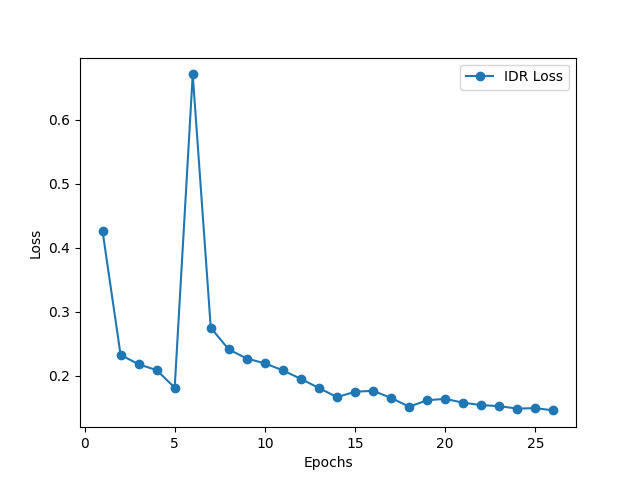
\includegraphics[width=\linewidth]{images/chapter5_img/LossPlots/Total_Loss_First_50-100_Epochs/loss_plot_PositionalEncoding.jpg}
        \caption*{Positional Encoding Loss Curve}
      \end{subfigure}
      \begin{subfigure}{0.3\textwidth}
        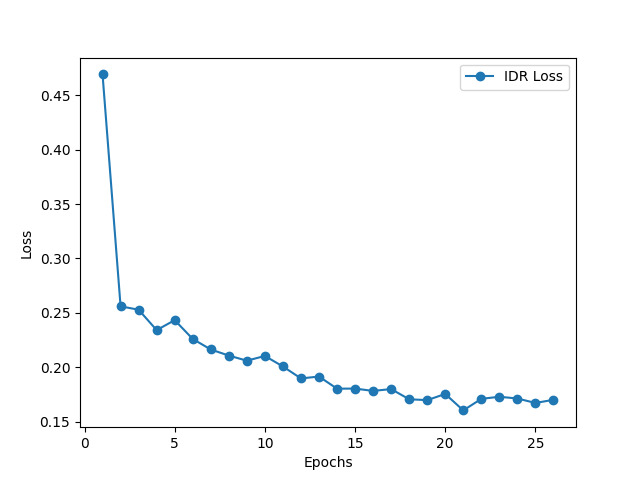
\includegraphics[width=\linewidth]{images/chapter5_img/LossPlots/Total_Loss_First_50-100_Epochs/loss_plot_FourierFeatures.jpg}
        \caption*{Fourier Features}
      \end{subfigure}
      \begin{subfigure}{0.3\textwidth}
        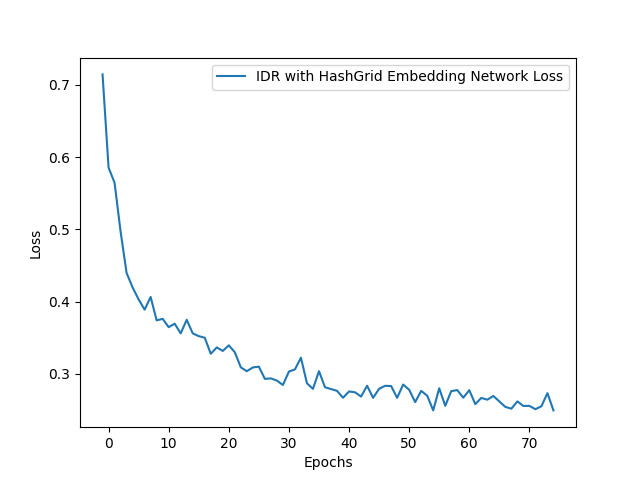
\includegraphics[width=\linewidth]{images/chapter5_img/LossPlots/Total_Loss_First_50-100_Epochs/loss_plot_HashGrid_EpochStamp75.jpg}
        \caption*{Multi-Res HashGrid 3D}
      \end{subfigure}
    
      \begin{subfigure}{0.3\textwidth}
        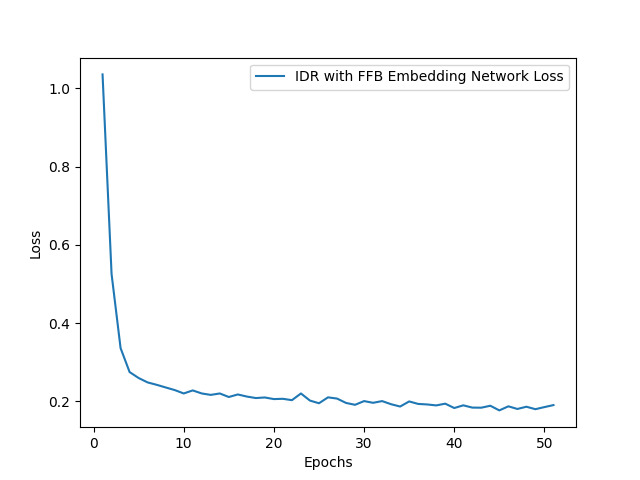
\includegraphics[width=\linewidth]{images/chapter5_img/LossPlots/Total_Loss_First_50-100_Epochs/loss_plot_FFB.jpg}
        \caption*{NFFB Loss Curve}
      \end{subfigure}
      \begin{subfigure}{0.3\textwidth}
        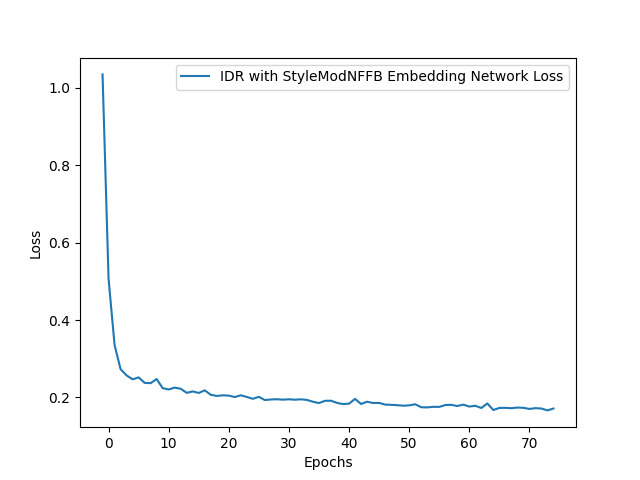
\includegraphics[width=\linewidth]{images/chapter5_img/LossPlots/Total_Loss_First_50-100_Epochs/loss_plot_StyleModNFFB_EpochStamp75.jpg}
        \caption*{StylemodNFFB Loss Curve}
      \end{subfigure}
      \begin{subfigure}{0.3\textwidth}
        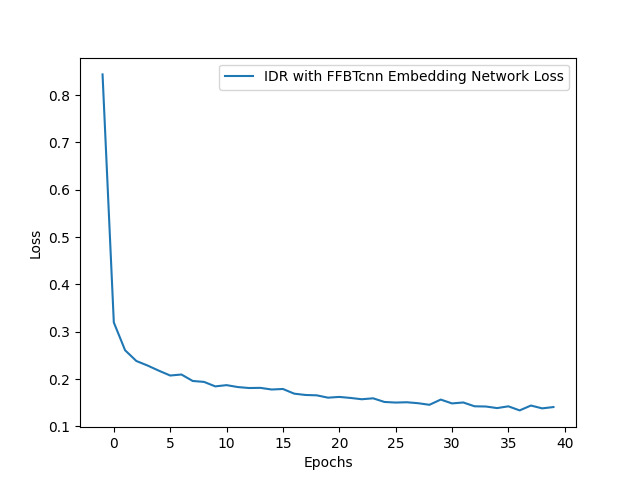
\includegraphics[width=\linewidth]{images/chapter5_img/LossPlots/Total_Loss_First_50-100_Epochs/loss_plot_FFBTcnn_EpochStamp40.jpg}
        \caption*{TCNN StylemodNFFB Loss Curve}
      \end{subfigure}
      \begin{subfigure}{0.3\textwidth}
        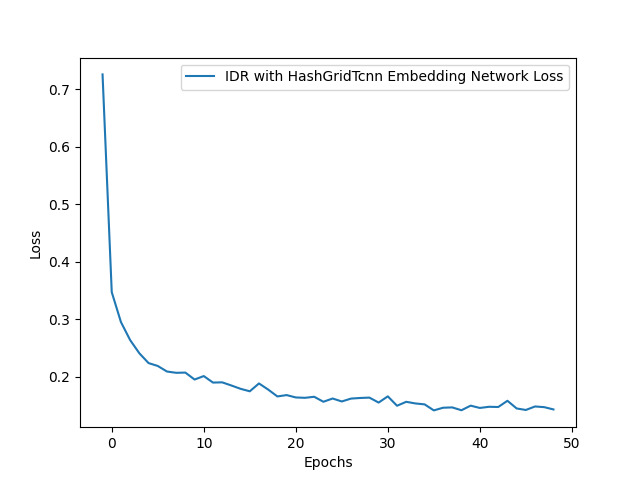
\includegraphics[width=\linewidth]{images/chapter5_img/LossPlots/Total_Loss_First_50-100_Epochs/loss_plot_HashGridTcnn_EpochStamp49.jpg}
        \caption*{TCNN MR-Hashgrid3D Loss Curve}
      \end{subfigure}
      \caption{Σύγκριση Σύγκλισης Αλγορίθμων στο Σφάλμα Εκπαίδευσης}
    \end{figure}
    H ταχύτητα σύγκλισης των αλγορίθμων θα μπορούσε να συγκριθεί με την κλίση των καμπυλών εκπαίδευσης και τα τελικά ορόσημα σφαλμάτων που επιτυγχάνονται στις 2000 εποχές εκπαίδευσης. Η εκπαίδευση που εκτελέστηκε ήταν διακοπτόμενη και με επανεκκινήσεις για λόγους ευστάθειας του εξοπλισμού αφού σε ορισμένες περιπτώσεις συσσωρεύονται τανυστές κλίσεων σφαλμάτων που υπερχειλίζουν την μνήμη καθώς οι υπολογισμοί γίνονται σε μεγάλο βάθος δικτύων. 
    \nobreak
\subsection{Σχόλια για την ταχύτητα των αλγορίθμων}
\par
      Οι αλγόριθμοι διαφέρουν ως προς τον χρόνο που ολοκληρώνουν την εκπαίδευση ξεκινώντας από του αλγορίθμους  κωδικοποίησης με πυρήνες Fourier να απαιτούν 24 ώρες για την ολοκλήρωση των 2000 εποχών ενώ το δίκτυο κατακερματισμού πολλαπλών αναλύσεων \enit{Multi-Resolution HashGrid3d} να χρειάζεται κάτι λιγότερο από μια μέρα για μία σκηνή του συνόλου δεδομένων. Σημαντική επιτάχυνση παρατηρείται στα πλήρως συγχωνευμένα δίκτυα κωδικοποίησης \enit{hash}, μέσω της βιβλιοθήκης \enit{TinyCUDANN}. Αυτά εκπαιδεύονται πλήρως σε λιγότερο από 14 ώρες.  Βέβαια αυτή η διαδικασία εκπαίδευσης είναι μια διαδικασία υπερεκπαίδευσης. Πρακτικά απαιτούνται 500 εποχές για να έχουμε ικανοποιητική αναπαράσταση.
 \subsubsection{Καμπύλες 2000 εποχών εκπαίδευσης}
    Ακολουθούν γραφήματα που παρουσιάζουν την συνολική πορεία όλων των επιμέρους σφαλμάτων ενδεικτικά για το δίκτυο NFFB. Παράγονται κατά την διάρκεια της εκπαίδευσης με χρήση του εργαλείου \enit{Tensorboard}.

    \begin{figure}[H]
      \begin{minipage}{0.5\linewidth}
        \centering
        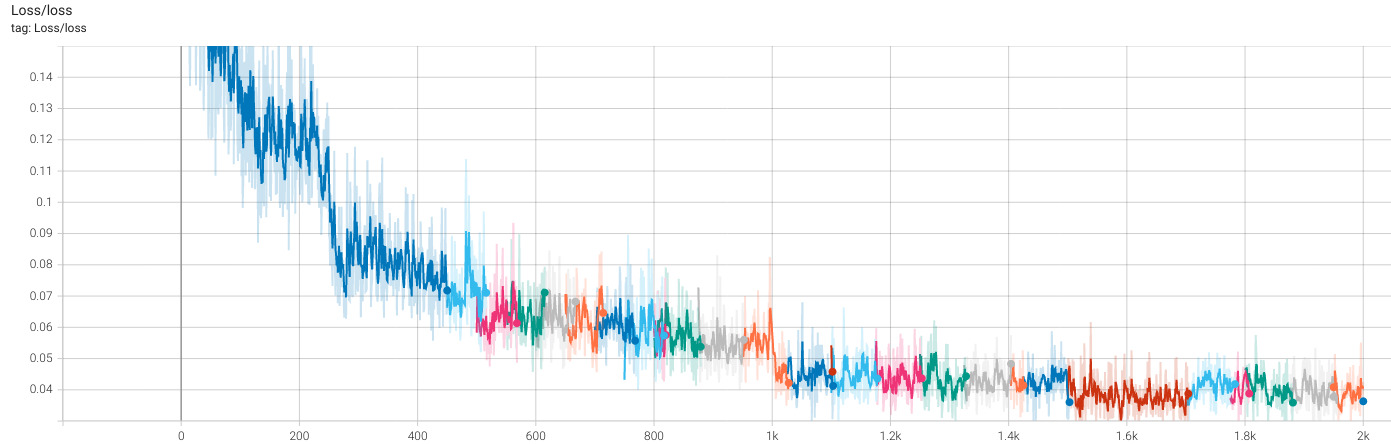
\includegraphics[width=\linewidth]{images/chapter5_img/LossPlots/Tensorboard_Losses/NFFB/NFFB_loss_PLot65.jpg}
        \subcaption{Συνολικό Σφάλμα}
      \end{minipage}%
      \begin{minipage}{0.5\linewidth}
        \centering
        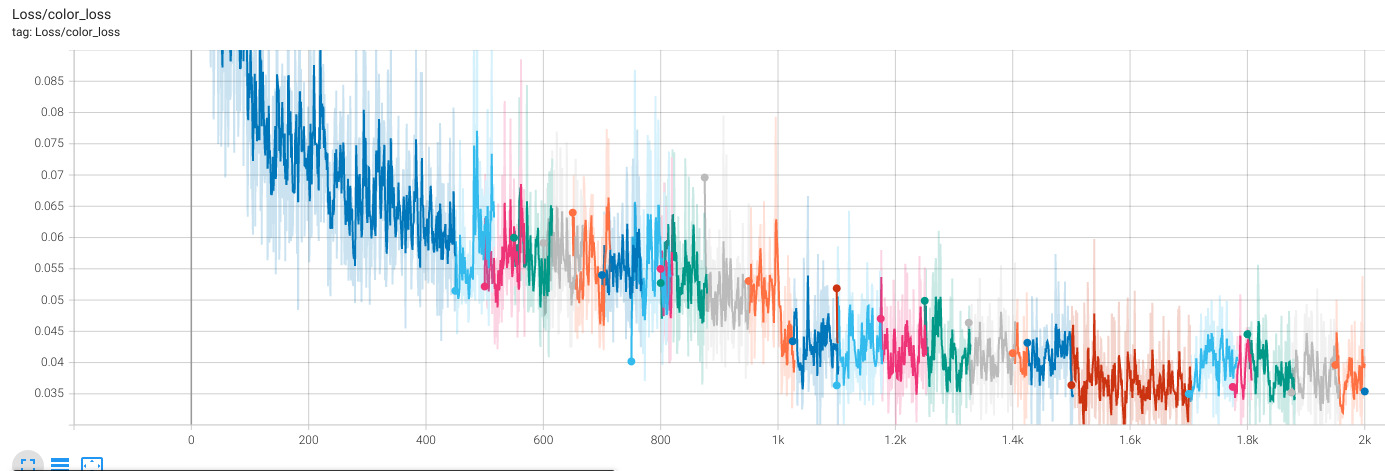
\includegraphics[width=\linewidth]{images/chapter5_img/LossPlots/Tensorboard_Losses/NFFB/NFFB_RGBloss_PLot65.jpg}
        \subcaption{Σφάλμα χρώματος εικόνας $L_1$, [R, G, B]}
      \end{minipage}
      \begin{minipage}{0.5\linewidth}
        \centering
        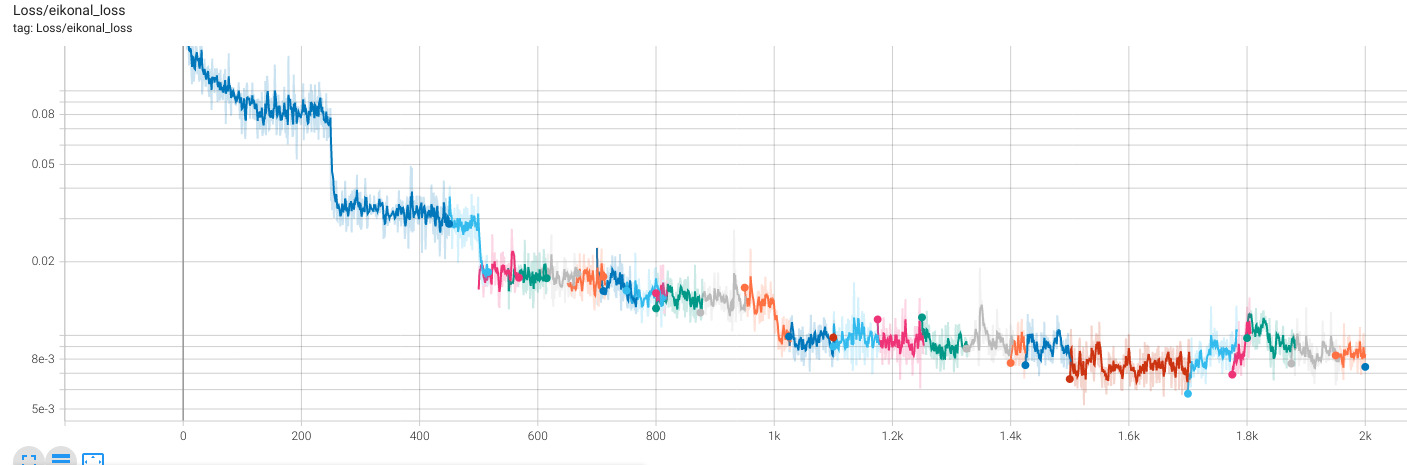
\includegraphics[width=\linewidth]{images/chapter5_img/LossPlots/Tensorboard_Losses/NFFB/NFFB_Eikonalloss_PLot65.jpg}
        \subcaption{Σφάλμα Εικονικής Εξίσωσης \enit{Eikonal Loss}}
      \end{minipage}%
      \begin{minipage}{0.5\linewidth}
        \centering
        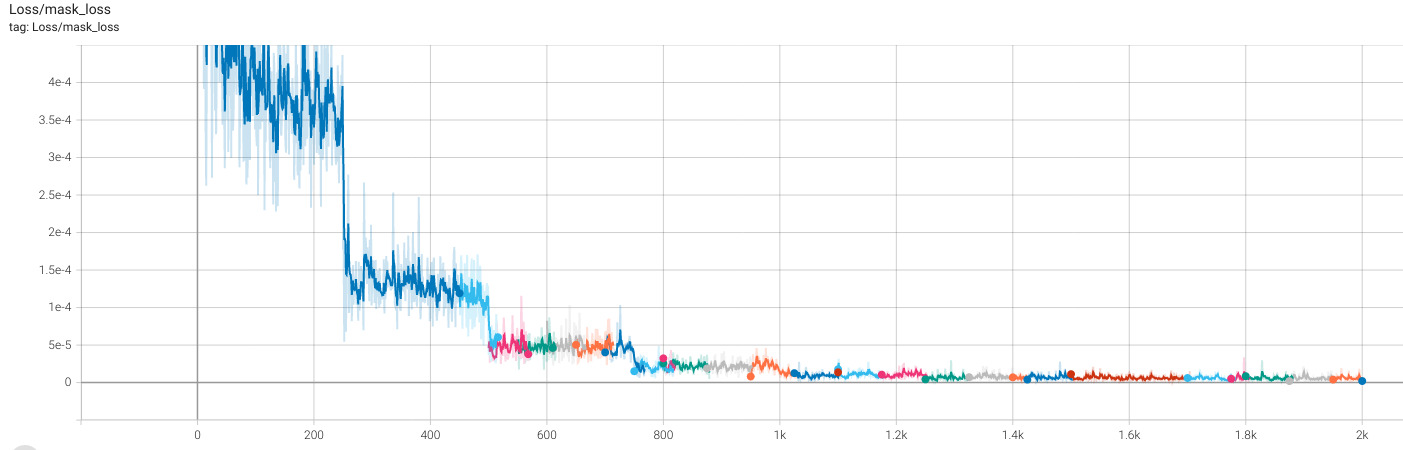
\includegraphics[width=\linewidth]{images/chapter5_img/LossPlots/Tensorboard_Losses/NFFB/NFFB_Maskloss_PLot65.jpg}
        \subcaption{Binary Cross Entropy - Σφάλμα μάσκας}
      \end{minipage}
      \caption{Καμπύλες Σφαλμάτων εκπαίδευσης NFFB, σε όλη την διάρκεια της εκπαίδευσης}
    \end{figure}

\subsection{Σχόλια για την αξιολόγηση}
\par 
      Η εκπαίδευση δεν κάνει διαχωρισμό των ομάδων pixel σε pixel εκπαίδευσης και pixel αξιολόγησης μιας και αυτό δεν είναι το ζητούμενο σε ένα πρόβλημα ανακατασκευής. Δηλαδή δεν είναι στόχος να κρύψουμε δεδομένα από το δίκτυο αποτύπωσης αλλά να καταφέρουμε να κάνουμε το δίκτυο να ελαχιστοποιήσει όσο το δυνατόν περισσότερο την αντικειμενική συνάρτηση βελτιστοποίησης με βελτιώνοντας όλα τα δίκτυα. Έτσι πρακτικά μπορούμε να πούμε πως όλες οι καμπύλες που παρουσιάζονται είναι καμπύλες που δείχνουν την σύγκλιση των συνεχών συναρτήσεων και το μεγαλύτερο μέρος αυτής της διαδικασίας φαίνεται στις πρώτες 50-100 εποχές.

     Η διαδικασία αξιολόγησης παράγει κυρίως τα αποτελέσματα μετρικών για την ανακατασκευή των μοντέλων χρησιμοποιώντας ως είσοδο τις ίδιες εικόνες επίβλεψης που χρησιμοποιούνται και στην εκπαίδευση. Είναι εφικτό να κρύψουμε ορισμένες εικόνες από το δίκτυο και να σπάσουμε το πρόβλημα σε δεδομένα εκπαίδευσης και δεδομένα αξιολόγησης ωστόσο αυτό δεν έχει ουσιώδες νόημα στα πλαίσια της ανακατασκευής, μιας και αντικειμενικός στόχος βελτιστοποίησης είναι να δημιουργηθεί μια υψηλής ακρίβεια ανακατασκευή με ήδη λίγα δεδομένα εκπαίδευσης.
    \nobreak